\chapter{Форматы данных для организации взаимодействия различных программно-аппаратных архитектур}\label{ch:ch3}

\section{Модель размещения данных.}\label{sec:ch3/sect1}

Для описания информации об эволюции численной модели была предложена базовая структура, хранящие данные о состоянии частицы как физические величины: позиция, скорость, ускорение, плотность, масса, вязкость, давление в каждый момент времени так и характеристические такие как идентификатор (\(particleID\)), идентификатор пространственной ячейки (\(cellID\)), тип частицы рисунок ~\ref{fig:p_struct}.
\begin{figure}[ht]
  \centerfloat{
    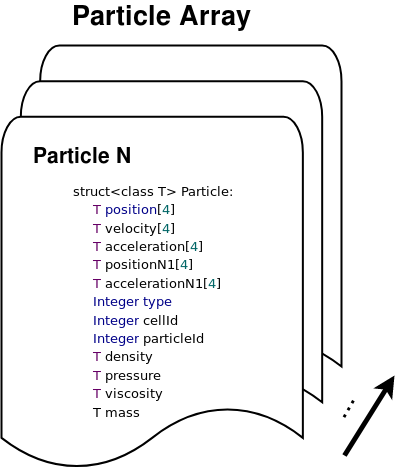
\includegraphics[scale=0.30]{p_struct}
  }
  \caption{Структура частицы.}\label{fig:p_struct}
\end{figure}

Таким образом модель описывается массивом частиц. При этом в зависимости от требования порядку точности вычислений можно варьировать обобщенный тип T между двумя интегральными типами данных \(float\) или \(double\). Каждая партиция определяется следующим образом пусть \(N\) – количество частиц \((p_0,...,p_{N-1})\) – упорядоченное по \(cellID\) множество начальных данных о частицах. Подразумевается, что каждый элемент \(p_i\) хранит пространственные координаты, координаты вектора скорости и \(cellID\) \(i\)-й частицы как показано на рисунке ~\ref{fig:p_struct}. Определим пространственные параметры модели 
\((x_{min}, y_{min}, z_{min})\), \((x_{max}, y_{max}, z_{max})\) – точки, определяющие границы области моделирования (вершины параллелепипеда, лежащие на его диагонали).
\(gridCellX\), \(gridCellY\), \(gridCellZ\)- количество пространственных ячеек по соответствующим измерениям трехмерного пространства. Эти значения получаются из целочисленного деления длины ребра ограничивающего объема на длину ребра пространсвенной ячейки например
\[
gridCellX = \left \lfloor \frac{\left |x_{max} - x_{min}  \right |}{2h} \right \rfloor
\]
\[
gridCellY = \left \lfloor \frac{\left |y_{max} - y_{min}  \right |}{2h} \right \rfloor
\]
\[
gridCellZ = \left \lfloor \frac{\left |z_{max} - z_{min}  \right |}{2h} \right \rfloor
\]
\(h\) – радиус сглаживания,
\(M\)– количество доступных устройств.

Для сравнительной оценки производительности устройства вводится эвристическая функция, которая рассчитывает коэффициент производительности на основе возможного количества потоков, которые можно одновременно запустить на конкретном устройстве:
\[
\epsilon(d_i)=D \cdot WG
\]
где \(d_i\) – устройство, \(D\)- количество доступных стриминговых мультипроцессоров (streaming multiprocessor - SM), для CPU – это число равно количеству ядер, \(WG\) – размерность рабочей группы для конкретного устройства. Например GPU Radeon R 290X обладает 44 стриминговых ядер, \(WG=256\).

Для достижения синхронности времени работы, необходимо, чтобы перед каждой итерацией данные были распределены между устройствами в количестве пропорциональном производительности устройств. Оптимальное количество частиц для обработки \(i\)-ым устройством определяется по следующей формуле:
\[
N_{i}^{'}=\left [ N \cdot \frac{\epsilon(d_i)}{\sum_{j}\epsilon(d_j)} \right ]
\]

Сформулируем еще два условия:
\noindent
\begin{enumerate}
  \item Все частицы, лежащие одной ячейке, должны обрабатываться одним устройством. Это условие можно сформулировать следующим образом:
\((C)\) \(\forall p_i, p_j\) \textit{если \(cellID\) частицы \(p_i=cellID\) частицы \(p_i\), то \(p_i, p_j\) обрабатываются одним устройством.}
  \item Количество пространственных ячеек обрабатываемых одним устройством должно быть кратным \(gridCellY\). 
\end{enumerate}

Следствием наложения этого условий является то, что итоговое количество частиц \(N_i \) для обработки \(i\)-м устройством  может отличаться от \(N_{i}^{'}\) (в зависимости от количества частиц в ячейке) т.е.:
\[
N_i = N_{i}^{'}+\Delta N_i, i=0,..., M-1 
\]
При этом:
\[
\sum_{j} N_j = \sum_{j}N_{j}^{'}=N
\]

Введем определение структуры партиции \(partition_i\) – структура для хранения индексов в общем массиве данных первой \(partition_{i}.start\) и следующей после последней частицы \(partition_{i}.end\), обрабатываемой \(i\)-м sudo snap install --classic goустройством с соблюдением условия 
\((C)\), которое достигается за счет упорядоченности множества частиц по номеру ячейки.  
\[
partition_{0}.start = 0
\]
\[
partition_{0}.end = partition_{0}.start + \epsilon (d_0) \cdot N + OFFSET_0 
\]
\[
...
\]
\[
partition_{i}.start = partition_{i-1}.end + 1
\]
\[
partition_{i}.end = partition_{i}.start + \epsilon (d_i) \cdot N + OFFSET_i, i=2,..., M - 1
\]
\(OFFSET_i\) – определяет количество частиц, которые находятся в добавочных ячейках (см. условие 2).
Заданные выше партиции определяют подмножества частиц, обрабатываемые соответствующими устройствами. Таким образом достигается распределение данных между устройствами так, что группы данных не пересекаются друг с другом. Как было уже сказано выше для корректности расчетов для частиц, которые находиться на границах партиций необходимо также учитывать частицы находящиеся в граничных ячейках соседних партиций.Устройство с номером  получает на обработку упорядоченный по  набор частиц. \fixme{К этому набору применяется параллельный метод PCI SPH. // тут нужно дописать}

\section{Модель вычислений.}\label{sec:ch3/sect2}

Модель вычислений определяет абстрактное представление того, как потоки инструкций выполняются в гетерогенной системе. Управляющая часть программы описывает, структуру, контролирующую ход вычислений и синхронизирует вычислительные узлы. Узел - отдельное независимое устройство GPU/CPU, обладающее изолированной памятью. В зависимости от количества узлов создается соответствующее количество параллельных потоков, выполняющих код отдельно, но в одном адресном пространстве. Каждый поток резервирует узел и контролирует вычисления на нем. Вычисления на узле могут проходить параллельно. Модель вычислений представлена на рисунке ~\ref{fig:calc1}.
\begin{figure}[ht]
  \centerfloat{
    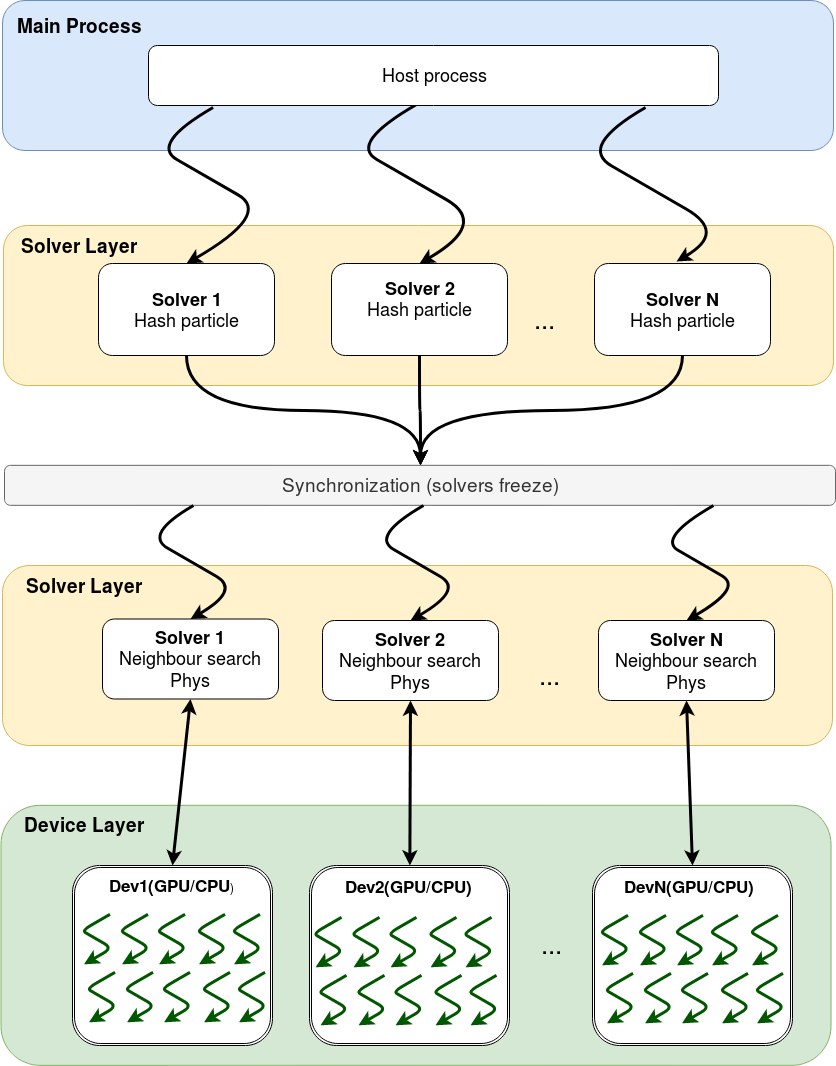
\includegraphics[scale=0.30]{calc1}
  }
  \caption{Модель вычислений.}\label{fig:calc1}
\end{figure}

Как видно из схемы, на этапе синхронизации все потоки  приостанавливаются, и управляющий поток синхронизирует данные между вычислителями, после чего вновь активирует их для дальнейшей работы. Синхронизация данных включает в себя процесс упорядочивания/сортировки массива частиц по соответствующему значению номера пространственной ячейки, актуализация массивов частиц в оперативной памяти устройств. 

Как показывают графики зависимости производительности от количества частиц для различных конфигураций время вычисления одной итерации моделирования сильно коррелирует с процессом синхронизации и, в значительной мере, сортировке \fixme{вставить ссылку на рисунок с графиками}. Для  конфигураций с количеством частиц, начиная от нескольких миллионов, сортировка может занимать до \(\sim \)50\% времени расчета итерации. В программной библиотеке sibernetic \cite{Palyanov2016} процесс упорядочивания может работать в двух режимах: параллельном и последовательном. 

При последовательном режиме используется быстрая сортировка quick sort \cite{Hoare1962}, реализованная в стандартной библиотеке шаблонов stl \cite{Stepanov1995} для языка программирования C++ \cite{Strosudo snap install --classic goustrup2013}. При этом асимптотическая сложность данного алгоритма равна \( O(N \cdot log(N)) \). Это позволяет довольно эффективно обрабатывать небольшие массивы до миллиона элементов и как показывают графики быстрее чем параллельная реализация. 

В параллельном режиме реализована модификация алгоритма цифровой сортировки предложенная в работах \cite{Knuth1998, Marcho1991}. Это позволило значительно ускорить процесс синхронизации как показано на рисунке \fixme{вставить ссылку на рисунок с графиками}. При этом асимптотическая сложность алгоритма равна \( 2^{r-1} \cdot O(\frac{N}{M}) \), где \( r \) - количество бит на один разряд для целого числа \( int32 \) это значение равно 4, \( N \) - количество элементов в массиве, \( M \) - количество потоков на вычислительном устройстве. Для того чтобы минимизировать количество перестановок в памяти комплексных структур, описывающих частицу ~\ref{fig:p_struct}, строится актуальная перестановка специального массива  индексов частиц, задающего взаимно-однозначное соответствие между текущим множеством и упорядоченным. Таким образом необходимость выделения избыточной памяти ограничивается лишь одним целым числом. 
Процесс переупорядочивания также выполняется параллельно.  На рисунке ~\ref{fig:sort1} показана. 
\begin{figure}[ht]
  \centerfloat{
    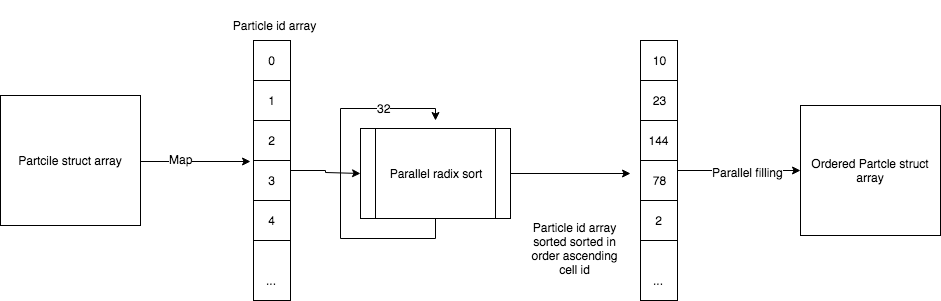
\includegraphics[scale=0.30]{sort1}
  }
  \caption{Схема работы процесса сортировки}\label{fig:sort1}
\end{figure}

\section{Параллельная реализация в системе программирования OpenCL.}\label{sec:ch3/sect3}

...

Для работы с параллельными вычислениями была выбрана платформа OpenCL, предназначенная для создания приложений, связанных с вычислениями на гетерогенных вычислительных системах, стандарт обеспечивает параллелизм на уровне инструкций и на уровне  данных и является реализацией техники GPGPU  \cite{Munshi2011, Stone2010}. Основными  преимуществами OpenCL являются открытость стандарта и поддержка большинством основных производителей как комплектующих, так и программного обеспечения, например Intel, AMD, NVIDIA, Apple (более подробный список на сайте http://www.khronos.org/opencl/). Таким образом это позволяет писать код, который можно запускать на различных устройствах GPU, CPU, FPGA. Код написанный на языке OpenCL интерпретируется соответствующим  компилятором, например, для GPU от компании NVIDIA компилятор OpenCL встроен в драйвер библиотеки CUDA \cite{Cook2012}.

Спецификация OpenCL интерпретирует любую платформу как хост-систему (host) и связанной с одним или более устройством, поддерживающим OpenCL. Каждое устройство состоит из одного или более вычислительных модулей - compute units,  которые  могут  включать  в  себя  несколько обрабатывающих элементов - processing elements. Вычисления  происходят  в обрабатывающих элементах устройства.

В данном контексте хост-система выступает в качестве контроллера, управляющего потоком  данных и конвейером вычислений. Обрабатывающие элементы модуля могут выполнять поток инструкций как единицы SIMD(single instruction, multiple data)\cite{Flynn1972} или как единицы SPMD(single program, multiple data streams)\citep{Darema2011}

вычислительной единицы (compute unit). Каждая вычислительная единица 

\fixme{все что написано дальше я спиздил, нужно переписать} \fixme{Спецификация OpenCL уходит от архитектурных различий, представляя любую плат-форму  в  виде хост-системы(h o s t),  связанной  с  одним или  более устройствами(d e v i c es). Каждое устройство состоит из одного или более вычислительных модулей(c o m p u t e    u n i t s),  которые  могут  включать  в  себя  несколько обрабатывающих элементов(p r o c e s s i n g   e l e m e n t s).  Все  вычисления  происходят  в  обрабатывающих элементах устройства. Очевидно, что столь общей моделью можно описать любые систе-мы, включающие центральные и графические процессоры, а также различные виды уско-рителей. Управляющее приложение запускается на хост-системе и передает команды OpenCLдля организации вычислений на устройствах. Обрабатывающие элементы одного вычис-лительного модуля могут выполнять поток инструкций как единицы SIMD(SingleInstruc-tion, MultipleData) или как единицы SPMD(ingle program, multiple data streams )1. Следует заметить, что часто пропускная способность внутренней шины вычислитель-ного устройства существенно выше пропускной способности шины, соединяющей его с хост-системой(типичная ситуация для графического процессора). Таким образом, переда-ча данных может занимать значительное время, и разработчик должен организовать до-статочный объем вычислений в каждом ядре, чтобы данный фактор не стал лимитирую-щим. Приложение на базе OpenCL включает в себя две компоненты: ядра(k e r n e l s),кото-рые  выполняются  на  устройствахOpenCL,  и управляющая  программа(h o s t  p r o g r a m), которая выполняется на хост-системе и организует исполнение ядер. Модель исполнения OpenCL определяет каждую компоненту. Исполнение ядер на устройстве.Перед запуском ядра определяется так называемое пространство  индексов(i n d e x   s p a c e).  Экземпляр  ядра  выполняется  для  каждой точки данного пространства и называется элементом работы(w o r k-i t e m). Соответ-ствующая точка в пространстве индексов задает его глобальныйидентификатор. Каж-дый элемент работы выполняет определенный путь внутри одного и того же кода, получая на вход уникальные данные.Такм способом реализуется параллелизм по данным, который является основным сценарием использования OpenCL.Элементы работы объединяются в группы  работ(w o r k-g r o u p), которые обеспе-чивают  более  крупнозернистую  декомпозицию  пространства  индексов.  Группам  работ также назначаются уникальные идентификаторы, размерность которых совпадает с раз-мерностью пространства индексов. В пределах одной группы работ каждый элемент по-лучает уникальный локальныйидентификатор. Таким образом, элемент работы опреде-ляется двумя способами: своим глобальным идентификатором или комбинацией локаль-ного идентификатора и идентификатора группы работ. Согласно  спецификации OpenCL,  элементы  работы, образующие группу  работ,  вы-полняются  на одномвычислительном  модуле.Стандарт  поддерживает  синхронизацию вычислениймежду элементами работы в одной группе работ с помощью механизма барь-еров. Синхронизация между различными группами работ и элементами работы в различ-ных группах напрямую не поддерживается. Стандарт  OpenCL  определяет N-мерное  пространство  индексов, однако в  текущей версии обеспечена  поддержка  для N=1,2,3. Данноепространство  задается  с  помощью массивацелых чисел длины N, который устанавливает его протяженность в каждом изме-рении. Глобальные и локальные идентификаторы элемента работы являются N-мерными кортежами. Компоненты глобального идентификатора принимают значения в диапазоне от нуля до числа элементов в соответствующем измерении минус один.Группам работ идентификаторы назначаются аналогично рассмотренной схеме: мас-сив длины Nопределяет число групп работ в каждом измерении. Элементы работы при-писываются к группамработ и получают локальныеидентификаторы, компоненты кото-рыхпринимают значения в диапазоне от нуля до размера группы работ в соответствую-щем измерении минус один.Как  можно  заметить,  модель  параллелизма OpenCLполностью  аналогична  модели NVIDIACUDA:  элемент работы соотвествует потоку,  а группа работ –блоку потоков. Однако  в  стандарте NVIDIACUDAвводится  понятие  сетки  блоков,  в  то  время  как  в OpenCLиспользуется пространство индексов, которое можно рассматривать как весь мас-сив элементов работы. Оба стандарта имеют механизмы индексирования, которые позво-ляют определитьместо конкретного экземпляра ядра в общем объеме работ. }
...

\section{Результаты тестирования и оценки.}\label{sec:ch3/sect4}

...

















